\documentclass[a4paper,twoside]{report}

% Enable UTF-8 text
\usepackage[utf8]{inputenc} % enable UTF-8 text

% Adds bibliography to table of contents
\usepackage[nottoc]{tocbibind}

% Automatically collect used acronyms
\usepackage[printonlyused,withpage]{acronym}

% Use newlines in paragraph instead of indentation
\usepackage{parskip}

% Adds the TODO package
\usepackage[backgroundcolor=white,linecolor=red,bordercolor=red]{todonotes}

% Build index
\usepackage{makeidx}
\makeindex

% Uncomment this if you want to show all \index{} locations in the document
% in the margins (good for proofreading)
%\usepackage{showidx}

% Hyperlinks, clickable references
% Hidelinks turns off colored box on some PDF viewers
\usepackage[hidelinks]{hyperref}

% On Mac OSX, in ViM, when I type ALT+SHIFT+SPACE (often typed accidentally
% after writing {\some-command ...}, then LaTeX may give me the error
% "Unicode char \u8:  not set up for use with LaTeX.".  This character
% in UTF-8 actually means what the tilde (~) means in LaTeX, but *I*
% usually mean just a space.  This command replaces those with a
% normal space:
\DeclareUnicodeCharacter{00A0}{ }
% If I really want the tilde-behaviour, I can use the command
%\DeclareUnicodeCharacter{00A0}{~}
%
% The above solution was taken from:
% http://tex.stackexchange.com/questions/83440/inputenc-error-unicode-char-u8-not-set-up-for-use-with-latex

\begin{document}
\author{Christian Stigen Larsen}
\date{Draft version: \today}
\title{Efficient Paxos on a software defined network\\\textsf{** DRAFT **}}
%\frontmatter % only for book document class
  \maketitle
  \listoftodos % TODO: Remove when finished
  \listoftables
  \listoffigures
  \tableofcontents
%\mainmatter % only for book document class
  \chapter{Introduction}

Around 2008, \textbf{\acf{SDN}}\index{software-defined networking}
\cite{Casado:2005:VNS:1047344.1047383} emerged from research at
Berkeley\index{Berkeley} and
Stanford\index{Stanford} as a way to enable networks to be defined and managed using
software. One model of \acs{SDN} is \textit{OpenFlow}\todo{Cite!}, which
decouples the control plane\index{control plane} from the forwarding
plane\index{forwarding plane}\index{data plane|see{forwarding plane}} in a
switch, moving it out of the physical switch to an external controller node.
It enables one to implement the controller in software.

Although invented quite recently, software-defined networking is already
being heavily used both in academia and industry.  Google\index{Google}, for instance, are
using OpenFlow to ease deployment and increase utilization in their backbone
networks\index{backbone network} \cite{crabbe2012sdn} and Stanford has deployed several
OpenFlow-controlled networks on their university network.

In March 2013, IDC\index{IDC} \todo{finn ut hva det står for} projected that the SDN market would
  reach \${}3.7 billion by 2016, capturing a 35\%{} share of the switching
  market \cite{Kirkpatrick:2013:SN:2500468.2500473}.
\todo{Skriv om denne setningen, den er tatt nesten direkte fra artikkelen!}

OpenFlow is detailed in \vref{chapter:background.openflow}.

\textbf{Paxos}\index{Paxos} \cite{Lamport:1998:PP:279227.279229} is a
family of distributed, fault-tolerant consensus algorithms.  It allows
network nodes to reach \textit{agreement} even in the face of intermittent
network failures.  For example, one can design a database system using Paxos
to make sure that transactions are executed in the same order on all nodes.

Originally published by Leslie Lamport\index{Lamport, Leslie} in 1989, Paxos
has spawned numerous extensions, including cheap Paxos,
\index{cheap Paxos}\index{Paxos!cheap Paxos} fast Paxos
\index{fast Paxos}\index{Paxos!fast Paxos} and Byzantine
\index{Paxos!Byzantine Paxos}\index{Byzantine Paxos}, fault-tolerant variants.

It is discussed in \vref{chapter:background.paxos}.

\textbf{Our aim} is to build an efficient, \textit{Paxos-enabled software defined
network}.  Paxos will be implemented on OpenFlow switches to guarantee that
packets sent to all of their connected nodes are sent in the same order.
These end-hosts can run any networking service and leverage the benefits of
Paxos without needing to handle any details of the algorithm.

\section{Hypothesis}

For simplicity, we will constrain our scope to a few primitives of
classic crash Paxos\index{Paxos!classic crash} in \textit{phase two},
where we have steady-state
flow\index{Paxos!steady-state flow} with no failures\index{Paxos!failure}.

Furthermore, we want to look at opportunities for increasing networking
performance by moving parts of the Paxos from the control
plane\index{control plane} down to the switches' forwarding
plane\index{forwarding plane}.

We will implement this in progressive stages:

\begin{enumerate}
  \item Implement Paxos entirely in controllers connected to an OpenFlow
  switch.

  \item Extend OpenFlow and Open vSwitch so we can execute Paxos in the
  forwarding plane of the switch.

  \item Move parts of the Paxos implementation down to the forwarding plane
  (OpenFlow \textit{flow tables}), achieving a good balance of performance and
  programming maintainability
\end{enumerate}

Our hypothesis is two-fold:

\begin{enumerate}
\item Network nodes can leverage Paxos guarantees \textit{transparently} by
implementing it on the software switches using OpenFlow.
\item We can achieve good relative performance by moving parts of the
implementation from the OpenFlow controllers down to the software switches.
\end{enumerate}

We aim to build a proof-of-concept system backing up these claims.  The
thesis will therefore be a study of \textit{feasibility}.

\section{Overview}

\todo{Flytt dette inn i teksten over, trenger ikke være egen section.}
We discuss the theoretical background needed to understand this thesis in
chapter \ref{chapter:background} \vpageref{chapter:background}.  If you already know \acs{SDN},
OpenFlow and Paxos, you can skip this chapter.

Then we look at what OpenFlow can offer us in chapter
\ref{chapter:details.openflow}
\vpageref{chapter:details.openflow}, detail what Paxos requires for
implementation in chapter \ref{chapter:details.simplified.paxos} 
\vpageref{chapter:details.simplified.paxos} and propose a
design based on this in chapter \ref{chapter:design} \vpageref{chapter:design}.
\todo{Sjekk at linker stemmer, kan gjerne forenkles også + forbedres}

Finally, we .... blabla ... look at benchmarks and conclude in chapter
\ref{chapter:conclusion} \vpageref{chapter:conclusion}.

\section{Scope}

\todo{Skriv mere og bedre}

We will only look at a simplified version of Paxos in which we only
implement accept and learn messages. We ignore liveness checking such as
heartbeats. We ignore implementing the expanded OpenFlow features in the
network protocol and controller. We only look at steady state Paxos.
We assume switches are co-located. etc etc etc.

We also ignore the fact that if a switch goes down and back up again, it
will need to rejoin the Paxos network and its end-hosts need to synchronize
state\index{synchronization} (or just copy the state from a host on another switch).

\section{Topology}

\todo{Kan kanskje flyttes opp til hypothesis? Vis først HVA vi vil gjøre, og
  så hypotese}

Here we present what we want to achieve.  First, let's look at the situation
for one switch\index{Paxos!topology}.

\begin{figure}[H]
  \centering
  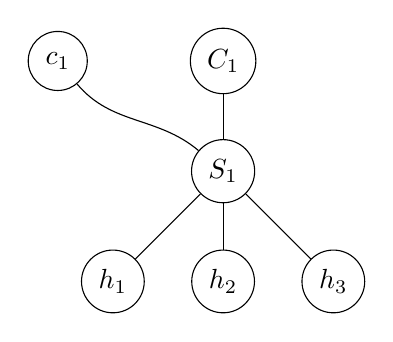
\begin{tikzpicture}[
      every node/.style={draw, circle, minimum width=0.75cm},
      x=0.7cm,
      y=0.7cm]
    \node (c1)    at (-3,  2) {$c_1$};
    \node (ctrl1) at ( 0,  2) {$C_1$};
    \node (S1)    at ( 0,  0) {$S_1$};
    \node (h1)    at (-2, -2) {$h_1$};
    \node (h2)    at ( 0, -2) {$h_2$};
    \node (h3)    at ( 2, -2) {$h_3$};

    \draw (c1) to[out=310,in=140] (S1);
    \draw (S1) -- (ctrl1);
    \draw (S1) -- (h1);
    \draw (S1) -- (h2);
    \draw (S1) -- (h3);

  \end{tikzpicture}
  \caption{A single switch $S_1$ with its controller $C_1$, end-hosts
    $h_1, h_2, h_3$ and one WAN-side client $c_1$.}
  \label{figure:graph.single.switch}
\end{figure}

For an explanation of our nomenclature\index{nomenclature}, we will always
talk about \textit{clients} as being remote hosts on the \ac{WAN} side.

The clients\index{client} are supposed to be placed on the \ac{WAN}---but they are actually
just ordinary hosts on each switch.  We just \textit{pretend} they are
placed on the \acs{WAN}\index{wide-area network}.  It really doesn't matter, though, as all of their
communication goes through each respective switch.

The \textit{end-hosts}\index{end-host} are nodes connected to a single
switch and running services such as key-value stores\index{key-value store},
lock-servers\index{lock-server}, logging servers\index{log server},
databases\index{database}, and so on.

Here is the situation with three switches---the minimum number nodes we need
in a Paxos system.  We have added all-to-all links between the switches in
case any one of them should go down.

\begin{figure}[H]
  \centering
  \begin{tikzpicture}[every node/.style={draw, circle},x=0.7cm,y=0.7cm]
    \foreach \n in {1,2,3} {
      \pgfmathsetmacro\x{(\n-2)*6}
      \node (c\n)    at (\x - 2,  2) {$c_\n$};
      \node (ctrl\n) at (\x ,  2) {$C_\n$};
      \node (S\n)    at (\x ,  0) {$S_\n$};

      \draw (c\n) to[out=305,in=125] (S\n);
      \draw (S\n) -- (ctrl\n);

      \foreach \h in {1,2,3} {
        \pgfmathsetmacro\pos{(\h - 2)*2}
        \pgfmathtruncatemacro\num{((\n - 1)*3) + int(\h)}
        \node (h\num) at (\x + \pos, -2) {$h_{\num}$};
        \draw (S\n) -- (h\num);
      }

    }

    % Links between switches
    \draw (S1) to[out=-10,in=190] (S2);
    \draw (S2) to[out=-10,in=190] (S3);
    \draw [dashed] (S1) to[out=-15,in=195] (S3);

  \end{tikzpicture}
  \caption{Three switches $S_1, S_2, S_3$ with controllers $C_1, C_2, C_3$ acting as Paxos nodes.
           The dashed line between $S_1$ and $S_3$ is a possible \textit{fail-over link}.}
  \label{figure:graph.three.switches}
\end{figure}
\todo{Merk at vi kommer til å ha én public IP-adresse for klienter! Så
      må kanskje vise det på en måte (eller bare nevne det)}

The point is that these services will be mirrored by the use of our
Paxos-enabled switches.  For our purposes, we will assume that the services
on these hosts are \textit{deterministic}\index{deterministic}\footnote{Or,
more correctly, \textit{referentially transparent}\index{referential
transparency}.} in the sense that the parameters uniquely determine the
state of the service after being processed---if two hosts running the
same service receive the exact same packet, their state will be
identical after having processed it.  This is a prerequisite for our
system.  The OpenFlow switches, running Paxos, will only make sure that
packets are delivered in the \textit{same order} to the end-hosts.

\section{Viability}

Why would such a system be useful? Consider the situation of implementing
Paxos in code on some servers, running services such as key-value
stores\index{key-value store}, etc.

\begin{figure}[H]
  \centering
  \begin{tikzpicture}[every node/.style={draw, circle},x=0.7cm,y=0.7cm]

    % For each switch ...
    \foreach \n in {1,2,3} {
      \pgfmathsetmacro\x{(\n-2)*6}
      \node (ctrl\n) at (\x ,  2) {$C_\n$};
      \node (S\n)    at (\x ,  0) {$S_\n$};

      \draw (S\n) -- (ctrl\n);

      % For each host ...
      \foreach \h in {1,2,3} {
        \pgfmathsetmacro\pos{(\h - 2)*2}
        \pgfmathtruncatemacro\num{((\n - 1)*3) + int(\h)}

        % Host node
        \node (h\num) at (\x + \pos, -2) {$h_{\num}$};
        \draw (S\n) -- (h\num);

        % Paxos node
        \node [very thick] (P\num) at (\x + \pos, -3.75) {$P$};
        \draw [dashed] (h\num) -- (P\num);
      }
    }

    % Links between switches
    \draw (S1) to[out=-10,in=190] (S2);
    \draw (S2) to[out=-10,in=190] (S3);
    \draw [dashed] (S1) to[out=-15,in=195] (S3);

  \end{tikzpicture}
  \caption{Support for Paxos on the servers $h_1, \dots, h_3$ requires a
    copy of the Paxos code $P$ on each server.}
  \label{figure:paxos.on.servers}
\end{figure}

Here, each server needs to have an implementation of Paxos in code (shown as
$P$ in figure \ref{figure:paxos.on.servers}).  It means the software
developer has to specifically add support for Paxos when designing the
server code, tailoring it for the particular service.  All Paxos handling
must be done at a high networking layer\index{networking layers}---most
likely in the application layer\index{application layer} at the very top.

Now consider the situation where the switch provides Paxos
capabilities\index{Paxos!on switch} (figure \ref{figure:paxos.on.switches}).

\begin{figure}[H]
  \centering
  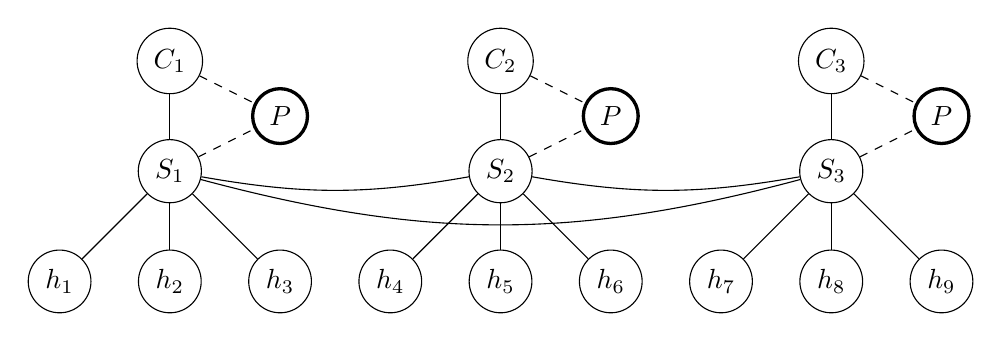
\begin{tikzpicture}[every node/.style={draw, circle},x=0.7cm,y=0.7cm]

    % For each switch ...
    \foreach \n in {1,2,3} {
      \pgfmathsetmacro\x{(\n-2)*6}
      \node (ctrl\n) at (\x ,  2) {$C_\n$};
      \node (S\n)    at (\x ,  0) {$S_\n$};

      \draw (S\n) -- (ctrl\n);

      % Paxos node
      \node [very thick] (P\n) at (\x + 2, 1) {$P$};
      \draw [dashed] (S\n) -- (P\n);
      \draw [dashed] (ctrl\n) -- (P\n);

      % For each host ...
      \foreach \h in {1,2,3} {
        \pgfmathsetmacro\pos{(\h - 2)*2}
        \pgfmathtruncatemacro\num{((\n - 1)*3) + int(\h)}

        % Host node
        \node (h\num) at (\x + \pos, -2) {$h_{\num}$};
        \draw (S\n) -- (h\num);
      }
    }

    % Links between switches
    \draw (S1) to[out=-10,in=190] (S2);
    \draw (S2) to[out=-10,in=190] (S3);
    \draw (S1) to[out=-15,in=195] (S3);

  \end{tikzpicture}
  \caption{Paxos ($P$) on the switches $S_1, S_2, S_3$ mitigates the need for special code on the servers.}
  \label{figure:paxos.on.switches}
\end{figure}

In figure \ref{figure:paxos.on.switches}, the switches themselves (and their
controllers\index{Paxos!controller}) enable
support for Paxos.\footnote{We have moved the servers to several switches
to indicate a distributed nature between the switches.
Paxos on a single switch would not be very useful, as that would be a single
point of failure and---after all---be the sole decision point for message
ordering.}
This should let the servers be oblivious of the fact that Paxos is used to
enable ordering of packet arrival to them.

Besides, Paxos is now run at a much lower networking level\index{networking
layers} and at the point where switching is done---there will be less hops
for each packet.

Of course, there are pros and cons for each scenario.
When implementing Paxos, one can often take advantage of
the particular way each server operates. Sometimes one actually
\textit{needs} to know this to implement Paxos.  Therefore, an
implementation of Paxos in each server's code base would be beneficial.

Also, it means that we need to run code on the switches themselves. This
gives rise to a wide range of non-functional requirements for the code.
For instance, code that runs for too long must be
preempted\index{preemption} to let the switch smoothly handle other
requests. Not doing so may result in packet loss, high latency or
worse---complete incapacity to serve data. Besides, switches do not normally
have hardware capable of running \textit{generic} software fast. They
usually have highly optimized hardware to do some of the heavy-lifting.

On the other hand, in our scenario, we can potentially add support for
message ordering through Paxos on servers that does not already support it.
The kinds of services that this would work on is for systems that are
deterministic in nature: The same input (or client packet) on any server
would produce the same internal state and output.
%
But there is a big class of software that has this behaviour:  Key-value
stores, logging servers, relational databases and so on.\footnote{But not
lock servers, because a lock can only be held by one server at a time.}

The only thing our model does not cover is the situation where a switch goes
completely down.
In that case, each connected server should start
synchronizing their internal state with any of the others that have been up.
\todo{Mangler jo også leader election og failures. Må få
  fram at jeg mener at KONSEPTET støtter mange ting, men ikke vår
    IMPLEMENTASJON.}

All in all, we believe this is a viable experiment with practical benefits.
Indeed, using a software-based approach for switches lets us test our model
on \textit{any} existing piece of server software.

Moreover, we also intend to show how one can optimize the performance of
this model further, by moving parts of the Paxos implementation down into
the switches' flow tables.  This should have a big impact, because Paxos
handling is done at a lower networking layer and closer to the central network
components than what would be the case with Paxos in the server's code.

\todo{Føler vi trenger flere, sterkere argumenter.}

  \chapter{Background}
\label{chapter:background}

In chapter \ref{chapter:introduction} we stated our thesis goal of offering
Paxos at the networking-level and building a distributed replication system
on top of it.
%
Here, we will present the background material for algorithms and technology
we will use in the rest of this thesis.

\section{OpenFlow}
\label{chapter:openflow.background}

As mentioned in chapter \ref{chapter:introduction}, the core idea of
\acs{SDN} is to dissociate the controller from the switch, enabling software
developers to ``program the network''.  This is illustrated in figures
\ref{figure:coupling.planes} and \vref{figure:decoupling.planes}.

OpenFlow \cite{McKeown:2008:OEI:1355734.1355746,openflow-1.0} is one of
several ways to enable \acf{SDN}
%
It is a specification of a messaging protocol for the interaction between
a switch and controller, detailing what kind of actions that can be
performed by each of these components.
%
Examples of \ac{SDN} solutions predating OpenFlow are SANE
\cite{Casado:2006:SPA:1267336.1267346}, Ethane
\cite{Casado:2007:ETC:1282427.1282382}, 4D
\cite{Greenberg:2005:CSA:1096536.1096541}.

In OpenFlow, the controller is a piece of software can inspect packets and
send commands down to the switch.  It can instruct the switch perform actions like
forwarding a packet to an output port going to another switch, changing
header fields, drop it and so on.
%
Additionally, the switch can be set up to perform such actions by itself,
using a \textit{flow table}.  This is what we have previously referred to as
the \textit{forwarding plane}, and as highly performant in comparison to
handling each individual packet in the controller.

OpenFlow controllers can be written in any programming language that offers
an OpenFlow framework.  While the OpenFlow switches are usually also
implemented in software, several vendors now ship hardware switches that
support the OpenFlow protocol.

\subsection{The Flow Table}
\label{chapter:theory.flow.table}

The aforementioned flow table consists of several flow
entries---colloquially called \textit{flows}.
%
These contain rules for matching packets and actions to perform when there
is a match.
%
In addition there are several counters used for collecting various
statistical metrics (e.g., how many times a flow has been executed) and
timeouts that dictate how long an entry will exist in the table.

\begin{figure}
  \centering
  \begin{subfigure}[t]{0.45\textwidth}
    \centering
    \begin{tikzpicture}[every node/.style={draw, circle},
                        node distance=2.5cm]
      \node [rectangle,
             rounded corners,
             minimum width=3cm,
             minimum height=1cm] (Sbig) at (0,0) {};

      \node [draw=none] (S) at (0,0) {$S$};
      \node [right=0.25cm of S] (C) {$C$};
      \node [left=0.25cm of S] (F) {$F$};

      % Add invisible node from figure B so that they align vertically
      \node [draw=none] (vspacer) [above of=S] {};

      \node (h1) [dashed, below left of=S] {};
      \node (h2) [dashed, below of=S] {};
      \node (h3) [dashed, below right of=S] {};

      \draw [dashed] (Sbig) -- (h1);
      \draw [dashed] (Sbig) -- (h2);
      \draw [dashed] (Sbig) -- (h3);

    \end{tikzpicture}
    \caption{A typical switch $S$ combines the control and
      forwarding planes ($C$ and $F$) on the same device.
        The control plane
        $C$ is usually locked down by the vendor and inaccessible to users.}
    \label{figure:coupling.planes}
  \end{subfigure}%
  \hspace*{0.1\textwidth}%
  \begin{subfigure}[t]{0.45\textwidth}
    \centering
    \begin{tikzpicture}[every node/.style={draw, circle},
                        node distance=2.5cm]

      \node [rectangle,
             rounded corners,
             minimum width=3cm,
             minimum height=1cm] (S) {$S$};

      \node (T) [above of=S] {$C$};
      \node (h1) [dashed, below left of=S] {};
      \node (h2) [dashed, below of=S] {};
      \node (h3) [dashed, below right of=S] {};

      \node (FlowTable) [left=-0.9cm of S] {$F$};

      \draw (T) -- (S);
      \draw [dashed] (S) -- (h1);
      \draw [dashed] (S) -- (h2);
      \draw [dashed] (S) -- (h3);

    \end{tikzpicture}
    \caption{\ac{SDN} decouples the control plane $C$ from the forwarding
      plane $F$ by moving it out of the switch $S$ to an external network
        node.  The \textit{OpenFlow protocol} enables communication between
        $S$ and $C$, making it possible to implement $C$ in software on an
        ordinary computer. In OpenFlow, the connection between $S$ and $C$ is encrypted.}
    \label{figure:decoupling.planes}
  \end{subfigure}
\end{figure}

When a switch receives a packet, it will try to match it with entries in
the flow table (table \vref{openflow.flow.entry.spec}).
%
Each flow contains a \textit{matching pattern}\index{OpenFlow!matching} and
a set of actions\index{OpenFlow!actions}\index{flow table} to perform in
case there is a match.
%
The actions can be to rewrite a header field, forward the
packet to a port, drop it and so on.
%
If a packet does not match any flows, the switch will forward a buffer ID
and packet headers to the controller $C_1$ on a secure channel.

\begin{table}[H]
  \centering
  \begin{tabular}{|c|c|c|}
    \hline \textbf{Header fields} &
           \textbf{Counters} &
           \textbf{Actions} \\
    \hline \dots & \dots & \dots \\
  \end{tabular}

  \caption{The OpenFlow 1.0 flow table.}
  \label{openflow.flow.entry.spec}
\end{table}

The controller can then decide what to do with the packet.  Using the
OpenFlow protocol, it can issue immediate actions to the switch or install
flows, so the switch can operate on its own.

The flow tables are initially empty, meaning that all packets are by default
sent to the controller.  During this phase, the controller will
explicitly handle every packet.  At the same time, it will incrementally
build up an internal map of the network.  As the map forms, it can start
installing flows in the switch.

For instance, if a controller learns the port numbers for a pair of
addresses, it can instruct the switch to automatically forward packets to
their appropriate output ports when they communicate.
%
If a packet's destination port is unknown, the controller can
\textit{rebroadcast}\index{rebroadcasting} it out on all ports except where
it came from, knowing that only designated receivers will accept the packet.
%
What we have described here is a \textit{learning switch}, and is explained
in detail in chapter \vref{chapter:l2.learning.switch}.

Along with each flow entry is an associated set of timeouts.  Flows are
removed from the flow table when they time out.
%
This serves several purposes.  First of all, it makes sure that flow tables
do not fill up quickly.  Secondly, because flows---and packets---are
transient by nature, controllers will be given the chance to update rules
based on changes in the network.
%
Finally, this mode of operation adheres to the principle of autonomous
operation\index{autonomous operation} commonly seen in networking devices.

Well-designed controllers should not need elaborate configuration to work.
So while they initially do all the heavy-lifting by themselves, they will
offload work to the switches, who can then dispatch packets very quickly.

\subsection{Applications of OpenFlow}

We would like to briefly mention a few real-world uses of OpenFlow.

Researchers at Stanford\index{Stanford}
built an OpenFlow network that was able to migrate a virtual video game
server \ac{VM} from California to Japan---while it was running, without
interruption, using the \textit{same} IP-address
\cite{erickson2008demonstration} \cite{kobayashi2013maturing}.

Google are using OpenFlow in their backbone network to increase utilization
\cite{crabbe2012sdn} and is an official member of the governing institution
of OpenFlow, the \ac{ONF}.

The Open Networking Foundation released the first specification of OpenFlow
in 2009 and continually publish point versions, errata and new versions
\cite{openflow-1.0,openflow-1.0.1,openflow-1.0.2,openflow-1.1,openflow-1.2,openflow-1.3,openflow-1.4}.
The most recent one, at the time of writing, is version
1.4\index{OpenFLow!versions}.

\section{Mininet, POX and Open vSwitch}
\label{chapter:mininet}

Mininet \cite{github:mininet} is an open source network simulator that
supports OpenFlow.
%
Using the Python programming language, one can deploy virtual networks on a
laptop, configuring link speeds, percentage of packet loss and so on.
%
Controllers are written using the POX \cite{github:pox} OpenFlow framework.

At the bottom of all this is the Open vSwitch program \cite{github:ovs}.
It is a powerful software switch used by many cloud providers.
It supports most of the OpenFlow functionality, and runs both as a Linux
kernel module and in user space.
%
Open vSwitch is written by many of contributors of the OpenFlow
specifications, and the three projects share close ties.

Together, they form a powerful combination of software that makes it easy
to experiment with networking technology.  We have used them for our thesis
implementation.

\section{Paxos}
\label{chapter:background.paxos}

Paxos \cite{Lam01, Lamport:1998:PP:279227.279229} is a family of
fault-tolerant, distributed consensus algorithms, allowing nodes to reach
agreement in the face of intermittent failures.
%
Originally published by Leslie Lamport\index{Lamport, Leslie} in 1989, Paxos
has spawned numerous extensions, including cheap Paxos,
\index{cheap Paxos}\index{Paxos!cheap Paxos} fast Paxos
\index{fast Paxos}\index{Paxos!fast Paxos} and Byzantine
\index{Paxos!Byzantine Paxos}\index{Byzantine Paxos}, fault-tolerant variants.

We will not give a full account of the Paxos algorithm here, but will
mention the main parts that are relevant for this thesis.  For reference, we
will hereafter keep to the description given in \cite{Lam01}.

Paxos consist of two main phases: \textit{Phase one} and \textit{phase 2}.
The first phase consists of choosing a leader among all the Paxos nodes.
This phase continues until a leader has been chosen by the majority.
As we will only focus on phase two, we will not discuss this part further.

Phase two, also called \textit{steady-phase}, is where \textit{message
ordering} takes place.   We say that we want to reach \textit{consensus} on
some \textit{value}.  A \textit{value} can be anything we want a majority of
the nodes to agree on.  For our purposes, it means we want to determine
which packet to next process (i.e., we want to determine the
    \textit{order} in which to process packets).  Paxos nodes will send
Paxos messages to each other, and they contain various parameters.  We will
return to these in section \vref{section:paxos.consensus.algorithm}.

The \textit{Paxos leader} from the first phase will receive a message
somehow---in our case, it will be a client packet that we wish to distribute
and process in-order---send out an \textit{accept} message containing a
\textit{value} to be agreed upon---the value can for example be a packet or
a reference to a packet, for example---and sending out an \textit{accept}
message to its \textit{Paxos slaves}.  Only the leader sends out accept
messages.

When a slave received an accept, it will first see if this is a message that
came from its current leader.  If so, and if it has not seen this message
before, it will send a \textit{learn} message to \textit{all} Paxos nodes,
including itself.

Upon receiving a learn-message, a node will first check if it belongs in the
current \textit{round}---meaning that the message belongs in the current
round with the given leader.  In other words, if the round number contained
in the learn message is less than the node's current round, this was a
message from a previous point in time in which there was
\textit{possibly} another leader.  If the learn has not been seen before, it
will record how many unique learns it has seen.
%
Whenever a node has received learns from a majority of other nodes, it will
start to process a queue of messages in the order specified by the message
parameters.

We will refrain ourselves from discussing \textit{why} the algorithm works,
even in the face of failures.  For such details, we refer to \cite{Lam01,Insane.Paxos}.

This concludes our very brief account of Paxos, and we will return to it in
section \ref{section:paxos.consensus.algorithm}.

  \chapter{OpenFlow}
\section{Features in OpenFlow versions 1.0--1.4}

To see how we can enable Paxos functionality in OpenFlow, we need to take a
look at what features it can provide us.

Naturally, we could implement the whole Paxos algorithm in the controller
itself.  Doing so should be quite trivial: One could take an existing
implementation and make some slight modifications to it.  There is in fact
some merit to this idea, because we could deploy systems where most of the
Paxos algorithm is implemented on the controllers, leaving some minor Paxos
code to run on the end--systems (for instance, the end--systems would need
to recognize Paxos LEARN--messages and extract the payload).

However, that would be very inefficient compared to running the entire
algorithm---or parts of it---on the switch.

OpenFlow controllers are meant to set up entries in the flow tables as they
see fit.  In an efficient OpenFlow--system, the
controllers will initially get lots of packets and program the flow tables.
Over time, more work can be performed by the use of flow tables, and so the
controllers will only update the flow tables intermittently.

The flow tables themselves will then be able to match given
packets to the specification and perform actions on them.  These flow tables
are {\em designed} to allow very efficient implementations in hardware.  In
other words, this means that the actions that can be performed are very
simple and far from a fully--fledged programmable system.

Because of this, we need to take a look at what operations we can perform in
OpenFlow.  The versions vary quite a bit on this point, and a lot of
software only support given versions.  So let's get an overview of what is
possible in the different OpenFlow versions.




  \section{Paxos on the controller}

Our first step will be to implement simple Paxos \cite{Lam01} entirely in a
controller\index{controller}.

The aim is to show that a topology with a Paxos-enabled controller will
satisfy the requirements of Paxos---i.e.,~that nodes in the network reach
consensus with progress\todo{Skriv om, og sjekk at forklaring på reqs er
riktig}.

We will use Mininet\index{Mininet} \cite{Lantz:2010:NLR:1868447.1868466} to
run and simulate the \ac{SDN} and POX\index{POX} \cite{POX.1} for
implementing a Paxos in an OpenFlow controller.  POX is part of the
NOX\index{NOX}\index{controller!NOX|see{NOX}}-project \cite{Gude:2008:NTO:1384609.1384625}.  They both use
Python\index{Python}\footnote{Mininet uses Python version 2.7.}
\cite{vanRossum:2009:PRM:1610526} as the implementation language, which
means we can share some code between them.  Both projects are mature and
easy to use.  The Mininet simulation itself will run on a virtual machine
using VirtualBox\index{VirtualBox} \cite{Watson:2008:VBB:1344209.1344210}.

  \chapter{Paxos on the switch}

  \chapter{Extending the OpenFlow protocol}

  \chapter{Conclusion}
\label{chapter:conclusion}

\todo{Vis at vi har nådd målene våre, vis svakheter, vis benchmark, osv. Bør
  være en ganske kort oppsummering (max en side).}

\todo{Ta med at vi har sett vekk fra security, feks utnytting av
  algoritmene og sånt}

\appendix
  \chapter{Running the thesis code}
\label{chapter:install.vm}

The best way to run the thesis code is to download a virtual machine image.
We used VirtualBox\index{VirtualBox} for running this image, but it should
also work on VMWare\index{VMWare}.  It comes preloaded with
Mininet\index{Mininet}, Open vSwitch\index{Open vSwitch},
  POX\index{POX}\index{controller|seealso{POX}},
  Wireshark\index{Wireshark} and more.

The user \texttt{mininet} has password \texttt{mininet} and has
\texttt{sudo}-rights.

\section{Downloading and verifying the VM image}

The Linux\index{Linux} VM image containing a ready-to-run version of the
code in this thesis, along with all its tools, can be downloaded from

\begin{center}
  \url{http://csl.name/thesis/mininet-vm-x86_64.vmdk}
  \label{gpg:url}
\end{center}

To verify that this image has not been modified after the time of thesis
submission, you should download the author's GPG-key\index{GPG} (listing
\ref{gpg:key}, p.~\pageref{gpg:key}) and use it to verify the file digest
in (listing \ref{gpg:signature}, p.~\pageref{gpg:signature}).

To import the author's key, you can use \ac{GPG} or any software compatible
with PGP\index{PGP}.  Importing the key is done by running the command
\texttt{gpg --import} and pasting a copy of the author's key, ending the
input by hitting \texttt{CTRL+D}.\footnote{You can also copy the key to a
  file \texttt{key.asc} and importing it with \texttt{gpg --import key.asc}}
%
\begin{Verbatim}
$ gpg --import
# paste in author's key and hit CTRL+D
\end{Verbatim}
%
You should now see they key on your key-ring.
%
\begin{Verbatim}
$ gpg --list-keys
\end{Verbatim}
%
The key's fingerprint should be the same as below:
%
\begin{lstlisting}[label={gpg:key.fingerprint}]
pub   4096R/FA475DD2 2013-04-23 [expires: 2016-04-22]
      Key fingerprint = D611 0F24 4813 9908 1CFE  79BA 1AB4 2C77 FA47 5DD2
uid                  Christian Stigen Larsen (General key) <csl@csl.name>
sub   4096R/D2495ED9 2013-04-23 [expires: 2016-04-22]
\end{lstlisting}

Finally, you need copy the VM image digest (listing \ref{gpg:signature}
\vpageref{gpg:signature}) to a file called
\texttt{mininet-vm-x86\_{}64.vmdk.asc}, placed in the same directory as the
downloaded VM image \texttt{mininet-vm-x86\_{}64.vmdk} (from \vref{gpg.url}).
You can then run \texttt{gpg --verify mininet-vm-x86\_{}64.vmdk.asc} to verify
the digest against the author's key.\footnote{Note that if you haven't
marked the author's key as \textit{trusted}, you will get a warning about
it.  But it should say that the signature is good.}

\begin{Verbatim}
$ gpg --verify mininet-vm-x86_64.vmdk.asc
gpg: Signature made Thu Apr 24 11:52:02 2014 CEST using RSA key ID FA475DD2
gpg: Good signature from "Christian Stigen Larsen (General key) <csl@csl.name>"
\end{Verbatim}

\lstinputlisting[
  caption={GPG signature for the thesis VM image.},
  label={gpg:signature}]{mininet-vm-x86_64.vmdk.asc}

% This text is long and must be on its own page
\begin{lstlisting}[
  float,
  caption={The author's public GPG-key},
  label={gpg:key}]
-----BEGIN PGP PUBLIC KEY BLOCK-----
Version: GnuPG v1

mQINBFF21LABEACrXyM2pQ9rl0TFlubOUBb9OtUF+wxCIqFCCvgVoYNCbldXMixc
wJzv6y76m/xfrpzZjl73tAnbY3WezHpY5MtPc/OtaW0BL5nlx1i21tfoW4YpHF4N
jPXkLYFiglb43eChRE5xbH14iaJ335SLt4YKFMIArug6g9tBjyjkXvvZNXJOKxDr
jUFX13hIKzyF2x298j+sNwlXy8SUB1NM6NNrtmhD46QMqlxBn2/+U1gXQrDpBxJR
PlXomaiTNb9hEH2XQcTfPMnFbZTzGO2fWA/njzSRC3L5gwsbGronFbnkf0rN8RrF
amPOu171NsH5YhHbsVpGG6KepGA/i1zq9sPXXYHKC0NdOHdrGhEuOjDNWOy/hu0n
eldUclSmnL04QHIwGkZomrgyQT2GcNM0U5wyXZ4QHKjamNoT0etLpXPmXGMQhSVY
psVvchQfBzzohuiOqtb3KdbAqua09FB86AfmWOXsHnvv3A7q864QllpPhP0SwpZ/
bW9e/2POWYpaEZ1jWLkhj1ctnRDBP+2lvKu0zp8wvN4xRDVCPxHonbKhrWV0vCD7
UP+PAvqfhlgorXSeaSZvhMa4evSrYxZwYj52m3x3P5dSFDeFZFgrbJ/fNyRJRino
8dTYT/+ccEj1y+mGDPV2T0A60c+ZHmhpg1cshtOXk+c0qCfYEndmSAQT7QARAQAB
tDRDaHJpc3RpYW4gU3RpZ2VuIExhcnNlbiAoR2VuZXJhbCBrZXkpIDxjc2xAY3Ns
Lm5hbWU+iQI+BBMBAgAoBQJRdtSwAhsDBQkFo5qABgsJCAcDAgYVCAIJCgsEFgID
AQIeAQIXgAAKCRAatCx3+kdd0p8aD/9a6MBhfkanB4vZCKhNYjM89Oxo/E06zEAm
KCxy3N2TnRBkqwQFkflKVJe9nw2PsSITBbKDIVWV3jJ06Lgx+hVMyu5srvCPirSv
dF/0chS0tNL52ZIz13EJnprZZg80+CYPQoHPgOnS8xg+qV1bROFB5n4K+cyCy4Db
l36k316zZ042NwoaEMHqgLd7Lr55FpNyoHaGtGOLSmW4BQkfldx6G1kdJefFY43h
bj2YICuj6vY8ztmPVjrmtoiomMFAj+dIWW+z1TAsQ4lUhWpXEEIW5lNePBce2jVZ
1d+oWe9u//RzBRBKy/jI0GxE+Pq3ZdLOxM87tejYDcdb/QUQSGmQ4QugxvKXol5W
XT8wsfNm+c2amolnpVuWHMCHHZSY8PGLJwBc+oZOlEBrXxE8dU8uD3A3fBQgiABD
ETLEs0KzS9oo1m6EGrZSD0v3cbR4XtrEw9elUIhS6mwUpjoFqanNgwUXJiomsvjR
63FOw1wzO7TMz8weRr+ZUXMwvg7QEuxkIhGqnaAk5t1BMKNFneKs7NApwa2FyZ6q
oVZXG6INEee8Uw+SBph9jq9O2mBueiWVNei7+tHcZgqZAmNyPh1cwo37c4yHX707
hqzmdnnW54/HPDeIly4gC/wRQZUkWb5z981XiJgSLzppKdCyiX4ygJ730WdBjjYq
QW8ZING9xrkCDQRRdtSwARAA6xNB6yQIhYUkIZ1UfBq91iQIFrt6v0cxCUqCqFYG
y5+bnqOIoZqvNOW0oMPWKYNaCGow+lPFz8+alFBrrNzznoHYTQwNC68qaXxoIMH4
o4Ah+IK5KQ9g/iUu9fbCPcpFYH90z4TJM2uAeZO9eJQmQqaWqfj2Y9IFDNEgDEln
rq0BgpD1R+qArPsGT0i34wTQ+cO9apGZB8FH7bGqvqReBmifW9vHh7DVtA+og9Js
wWNJAaRCHv/AXnqfRxwCoeFQQGW4cncDDuaYvC6ADPPvQ9c6FzaFE36p45OKPzy/
Z1gAjDhs9dlkdtYxKj8uyMDBlDaC4J/rPfZ7kD2PFi0iXfEk0JyAXihaAjz3eJaH
xwnjRQVNrP4PW+3We3DI15VzgDmzjem2rVHBVigNhi5dFNbhSmTThQx2wRlOI57s
D3QDvJl+ppPHlP0yQETe4F9Op6diLm7jXHmvezII5RN29gKjgnz0jvXBKqHfXIco
SgB418Jp+XTzsuA/SuhuiOo/d0ac/RiM95pu8upYLbRo1VqJwQyTPqUzj0zWiSTl
waekJpwwkQONZwFtquYYVdLhR30X1GX92OfAd9JdbMGK7WR3RZfwNSUWKnCSbqoi
WAjHW9sEK7ltU8TKKXJjbseSPNKk9Khc8h87skmNofOknY03nTG50YTvHSWpxxdL
feEAEQEAAYkCJQQYAQIADwUCUXbUsAIbDAUJBaOagAAKCRAatCx3+kdd0npOEACU
Kw4AR5GBjBTcrb0JQj+YFBZO4heYA/4UMcbPqvwJzeX0nSuZ+vkB9GV08nd7/jC2
+CiHlTlrtoH40S7SdOGoZgNx7WHeHFKLo8i29lUf0ID55TOs0EctYwX/MWLWt8JJ
uZ8OXQnrXL9Mtg1yybkftMiqSmAYtWfcX6Wv86zpPzM8K4kWkd5o3NNFWBareEqL
fmdjNyyumpYX+5tHMc2v7oxG/oEC5SCVJmF5ZzFuiBBvJPPIxfYHajoR1Xz+kKf/
RDtbTJxnR0Ftfhwb5Tv4iX6rYXHwvC6bhKB4Knndba+WeN7tYKAX7rLEasdzubGj
vSZgJD3CZykk7WIq5exDHTw5E4BtgOZc5LxOf2KsWBxks6vdjbeAICA135tKxtDB
lPMytrCMNy6JNoA0fFB/KxSnOhOIxH4Ar/vXaBJxI0mQuhs9Qt+27alf6R6OgjIN
S7KQ5l3MaUFUaiRwvGJeeolT+e6X/ssLZQyWDkrNxkonZ+GhbSO5p5zgGXA3PXGg
X/18vQyTCn1jt+jzr+f/6BW+E9pqusJ4MYdDM5ThKv7TjyslMW71cdFjCHNkf1/k
9zduikQwVddgU4Ha3T6+jOY0VLncguA7UnMTOdFGdL4SchZjswDzOHPcOxC4+Un5
x7JoKcugqMAINWCfPKu5IXU6SqSkKA6ddVG/SJ5wcA==
=iAwm
-----END PGP PUBLIC KEY BLOCK-----
\end{lstlisting}
\clearpage % Clear page after this key as it's pretty long.

\section{Setting up the VM image}

The author's settings in \textit{VirtualBox}\index{VirtualBox|seealso{VM}}
for the Linux VM\index{VM!setting up} are given in table
\vref{table:vm.settings}.  The fields marked as \textit{needed} must be set
as shown, otherwise the VM may not work properly.

Start VirtualBox and create a new VM.  Then point to the provided VM image
(the option \textit{Use an existing virtual hard drive file})
and copy the settings in table \vref{table:vm.settings}.

When you boot the VM, you should try to ping a remote host on the internet,
then you should attempt to \texttt{ssh} into it from a terminal on the host
computer.

% TODO: Fix the VERTICAL spacing as well, it is still white
\begin{table}[ht]
  \begin{tabular}{!{\vrule width -1pt}c
                  !{\vrule width -1pt}l
                  !{\vrule width -1pt}l}
  \hline
    \textbf{Needed}    & \textbf{Field}       & \textbf{Value} \\
    \hline
                       & Name                 & mininet \\
\rowcolor{verylight} * & Operating system     & Ubuntu (64 bit) \\
                       & Base memory          & 1024 MB \\
\rowcolor{verylight} * & Boot order           & Hard disk \\
                       & Acceleration         & VT-x/AMD-V, Nested Paging \\
                       & Display Video memory & 16 Mb \\
                       & IDE Secondary Master & vboxguestadditions.iso \\
                       &                      & CD/DVD \\
\rowcolor{verylight} * & SATA Port 0          & \texttt{mininet-vm-x86\_{}64.vmdk} \\
\rowcolor{verylight} * &                      & Normal, 8,00 GB \\
\rowcolor{verylight} * & Network Adapter 1    & Intel PRO/1000 MT Desktop \\
\rowcolor{verylight} * &                      & NAT \\
\rowcolor{verylight} * &                      & MAC: \texttt{FEEDFACEBEEF} \\
\rowcolor{verylight} * & Network Adapter 2    & Intel PRO/1000 MT Desktop \\
\rowcolor{verylight} * &                      & Host-only Adapter, 'vboxnet0' \\
\rowcolor{verylight} * &                      & MAC: \texttt{0800270A8160} \\
    \hline
  \end{tabular}
  \caption{Author's settings for the VM image.}
  \label{table:vm.settings}
\end{table}
\index{VirtualBox|seealso{VM}}
\index{VM!VirtualBox settings}

It is important that you set up the network
\textit{exactly} as shown, otherwise it may not function correctly.\footnote{
  If it stil does not work, make sure you have set up the guest OS
    networking settings correctly (ch.~\vref{chapter:guest.settings}).
  You may also want to edit the file
  \texttt{/etc/udev/rules.d/70-persistent-net-rules}.
  Update the corresponding MAC address and comment out all other lines, then
  reboot the VM.
   You may also need to change the VM's IP-address in
  ch.~\vref{chapter:ssh.setup}. If unsure of the IP-address, type
  \texttt{ifconfig eth1 | grep inet} to see the VM's address.
}

The \texttt{vboxguestadditions.iso} is not needed. We have used it only to
enable sharing of folders between the VM and host computer.

Remember that you can log in using the user \texttt{mininet} with the
password \texttt{mininet}.  This user should be able to get a root shell by
typing \texttt{sudo bash}.

\subsection{Guest OS network settings}
\label{chapter:guest.settings}

To be able to use \acs{NAT} on your VM, you need to set it up on your guest
OS networking settings in VirtualBox.

In the VirtualBox manager, go to preferences, network, \textit{NAT Networks}
and add a \acs{NAT}-network called \textit{NatNetworking}. Use the settings
from table \vref{table:natnetworking.settings}.

You also need to add an entry under the tab \textit{Host-only Networks}
using the settings in table \vref{table:hostonlynetworks.settings}.

\begin{table}[H]
  \centering
  \begin{tabular}{ll}
    \hline \textbf{Field} & \textbf{Value} \\
    \hline
      Enable network & Yes \\
      Network name & NatNetwork \\
      Network CIDR & 10.0.2.0/24 \\
      Supports DHCP & Yes \\
    \hline
  \end{tabular}
  \caption{Settings for guest OS NAT networking.}
  \label{table:natnetworking.settings}
\end{table}
\index{VM!network settings}

\begin{table}[H]
  \centering
  \begin{tabular}{ll}
    \hline \textbf{Field} & \textbf{Value} \\
    \hline
      \textbf{Adapter} & \\
      Name & vboxnet0 \\
      IPv4 address & 192.168.56.1 \\
      IPv4 network mask & 255.255.255.0 \\
       & \\
      \textbf{DHCP server} & \\
      Enable server & Yes \\
      Server address & 192.168.56.100 \\
      Server mask & 255.255.255.0 \\
      Lower address bound & 192.168.56.101 \\
      Upper address bound & 192.168.56.254 \\
    \hline
  \end{tabular}
  \caption{Settings for guest OS Host-only Networks.}
  \label{table:hostonlynetworks.settings}
\end{table}
\index{VM!network settings}

\subsection{Setting up SSH}
\label{chapter:ssh.setup}

In order to work with the VM, you need to add the following optios to your
local \texttt{\~{}/.ssh/config}.

\begin{verbatim}
Host mininet
  Hostname 192.168.56.102
  User mininet
  ForwardX11 yes
  ForwardAgent yes
  RequestTTY yes
\end{verbatim}
\index{VM!ssh}

X11-forwarding\index{VM!X11 forwarding} is required in case you want to start xterms on Mininet
nodes or run Wireshark.\index{VM!Wireshark}  Note that it also forwards your
ssh-agent---you may not strictly need this.  The \texttt{RequestTTY}-option
is \textbf{very important}, because it lets us start terminal programs on the remote
host. Without it, some of the examples here will leave processes running in
the background on the remote host when you SIGINT them (CTRL+D).\footnote{If
you don't use this option, you can manually type \texttt{ssh -t} to request
TTYs correctly.}

You may need to change the \texttt{Hostname}-parameter for your particular
system.  Doing this correctly saves you time when the host computer changes
networks.

To be able to logon passwordless, you need to upload your public key:

\begin{verbatim}
$ cat ~/.ssh/id_rsa.pub | ssh mininet "cat - >> ~/.ssh/authorized_keys"
\end{verbatim}
\index{VM!ssh}

Boot the VM and make sure you can log on to it without typing a password:

\begin{verbatim}
$ ssh mininet
\end{verbatim}

\section{The thesis source code}

You can find the thesis source code on the Mininet VM under
\texttt{\~{}/bach}.

\section{Running the thesis code}

To start the first example...
\todo{Write instructions on how to run the thesis code here.}

\section{Building code}
\label{chapter:compiling}

\subsection{Open vSwitch}
\label{chapter:compiling.ovs}

To build Open vSwitch\index{compiling|seealso{Open vSwitch}}\index{Open
vSwitch!building} on the VM, do the following:

\begin{Verbatim}
# Remove the preinstalled ovs
$ sudo apt-get remove \
    openvswitch-common openvswitch-datapath-dkms
    openvswitch-controller openvswitch-pki openvswitch-switch

$ cd ~/ovs
$ ./boot.sh
$ ./configure --prefix=/usr \
              --with-linux=/lib/modules/`uname -r`/build

# To compile ovs
$ make
$ make test # optional; takes some time

# To install
$ sudo make install
$ sudo make modules_install
$ sudo rmmod openvswitch
$ sudo depmod -a

# Now restart Open vSwitch
$ sudo /etc/init.d/openvswitch-controller stop
$ sudo /etc/init.d/openvswitch-switch stop

# Disable start of controller on boot
$ sudo update-rc.d openvswitch-controller disable

# And start again
$ sudo /etc/init.d/openvswitch-switch start

# Check that it's running
$ ps auxwww | grep openvswitch

# The executable ovs-controller changed name to test-controller
# in a recent ovs version, and Mininet relies on it:
$ sudo cp tests/test-controller /usr/bin/ovs-controller

# Check the version
$ sudo ovs-vsctl show
cd702e96-d4af-4803-9e2f-ecc2f7abcd6a
    ovs_version: "2.1.0"

$ modinfo openvswitch
filename: /lib/modules/3.8.0-35-generic/kernel/net/openvswitch/openvswitch.ko
license:        GPL
description:    Open vSwitch switching datapath
srcversion:     15C32AD9E04F379CAC3D68E
depends:
intree:         Y
vermagic:       3.8.0-35-generic SMP mod_unload modversions
\end{Verbatim}

\subsection{POX}

\todo{hvordan kompilere pox}

\subsection{Thesis code}

The thesis code is mostly written in Python, so no steps are necessary.
The only thing to remember is to use the correct PYTHONPATH.  You are
recommended to use the makefiles for this. We have also added symlinks where
needed, so you should not need to worry about it.

\todo{Hvordan bygge koden vår, C-koden, osv.}

\section{Running the benchmarks}
\label{chapter:appendix.benchmark}

To run the benchmarks yourself, you first need to set up the Linux VM image
by following the instructions in \ref{chapter:install.vm}
\vpageref{chapter:install.vm}.

You absolutely need to have set up \texttt{ssh} as shown in
\ref{chapter:ssh.setup} \vpageref{chapter:ssh.setup}, because we need
correct allocations of TTYs.

When you have done that, you may want to restart your Mininet before running
benchmarks.  This is to make sure that no processes from previous runs are
hanging in the background.\footnote{There may even be hanging processes from
the time the VM image was uploaded.} The test code mostly takes care of
this, but to be on the safe side, reboot with

\begin{Verbatim}
$ ssh mininet
$ sudo shutdown -r now
\end{Verbatim}

\subsection{Baseline benchmark}
\label{chapter:appendix.baseline.benchmark}

To run this benchmark\index{benchmark}, run the following on your local computer

\begin{Verbatim}
$ ssh mininet make bench-baseline
$ ssh mininet make bench-baseline-noflows
\end{Verbatim}

If you prefer to run Mininet and the controller in separate terminals, you
can start each one independently:

\begin{Verbatim}
# Terminal 1 (start first)
$ ssh mininet make bench-baseline-pox

# Terminal 2 (start after POX is up)
$ ssh mininet make bench-baseline-mininet
\end{Verbatim}

After the test runs complete, there are two result files that you can
download locally:

\begin{Verbatim}
$ scp mininet:~/pings.txt mininet:~/pings-noflows.txt .
\end{Verbatim}

  \chapter{Acronyms}
\begin{acronym}
\acro{ICMP}{Internet Controll Message Protocol}
\acro{IP}{Internet Protocol}
\acro{L2}{OSI link--layer}
\acro{NIC}{Network interface controller}
\acro{QoS}{Quality--of--service}
\acro{RPN}{Reverse Polish notation}
\acro{SDN}{Software--defined networking}
\acro{TCP}{Transmission control protocol}
\acro{TLS}{Transport Layer Security}
\acro{TOS}{Top of the stack}
\acro{ToS}{Type--of--service}
\acro{UDP}{Uniform Datagram Protocol}
\acro{VM}{Virtual Machine}
\acro{WAN}{Wide--area network}
\end{acronym}

%\backmatter % only for book document class
  \bibliography{bibliography/sdn,bibliography/paxos,bibliography/software,bibliography/mininet,bibliography/openflow}
  \bibliographystyle{plain}
  % Because of hyperref/makeidx/toc bug, we have to insert anchors ourselves
  % here. See
  % http://tex.stackexchange.com/questions/138903/wrong-hyperref-for-index-in-tableofcontents-since-texlive-2010
  \clearpage
  \phantomsection
  \printindex
\end{document}
